\chapter{Softwaretests} \label{chap:softwaretests}

In diesem Kapitel wird auf die Evaluierungs- und Testvorgäne für die Sicherstellung der Güte der entwickelten Software eingegangen.
Da es sich bei der entwickelten Software um ein Machine-Learning-Modell handelt, wird in diesem Kapitel auf die Evaluierung des Modells eingegangen. Die Funktionen des interpretierten Python Skripts entwickeln keine neuen Algorithmen, die auf ihre Fehleranfälligkeit oder Korrektheit getestet werden müssen.

\section{Metriken zur Evaluierung} \label{sec:metriken}

Um zu verstehen wie ein Machine Learning Modell evaluiert werden kann ist es zunächst wichtig die Arten von Kriterien nachzuvollzihen, die für die binäre Klassifikation notwendig sind. Im Folgenden wird allgemein von Instanzen gesprochen, es handelt sich dabei um die Bilder, der PCBs die klassifiziert werden sollen.

\begin{itemize}
    \item \textbf{True Positive (TP)}: Die Anzahl der korrekt klassifizierten positiven Instanzen.
    \item \textbf{True Negative (TN)}: Die Anzahl der korrekt klassifizierten negativen Instanzen.
    \item \textbf{False Positive (FP)}: Die Anzahl der falsch klassifizierten positiven Instanzen.
    \item \textbf{False Negative (FN)}: Die Anzahl der falsch klassifizierten negativen Instanzen.
\end{itemize}

Diese wesentlichen Typen teilen die Klassifizierten Daten nach dem Test in vier diskrete Kategorien ein. Diese Kategorien bilden die 
in \autoref{sec:confusionmatrix} beschriebene Confusion Matrix. Mit Ihnen können aber auch die Einfacheren Werte Loss und Accuracy berechnet werden. Im Folgenden wird die Mathematik hinter den Methoden vorgestellt.

\subsection{Accuracy und Loss} \label{sec:accuracy}

Die Accuracy ist eine der einfachsten Metriken zur Evaluierung eines Machine-Learning-Modells. Sie gibt an, wie viele der Instanzen korrekt klassifiziert wurden. Die Accuracy wird vereinfacht wie folgt berechnet:

\begin{equation}
    \text{Accuracy} = \frac{n_{\text{richtig klassifiziert}}}{n_{\text{gesamt}}}
\end{equation}

Bezug auf die in \autoref{sec:metriken} beschriebenen Kategorien, kann die Accuracy wie folgt berechnet werden \cite{ai_wiki_accuracy_2019}:

\begin{equation}
    \text{Accuracy} = \frac{TP + TN}{TP + TN + FP + FN} 
\end{equation}

Die Accuracy wird typischerweise in Prozent angegeben und liegt zwischen 0 und 100\%. Sie ermöglicht eine schnelle Einschätzung der Modellgüte. Allerdings kann die Accuracy irreführend sein, da sie die Anzahl der falsch klassifizierten Instanzen nicht berücksichtigt. Ein Modell, das alle Instanzen als negativ klassifiziert, könnte eine hohe Accuracy aufweisen, obwohl es nicht leistungsfähig ist.

Dennoch ist die Accuracy einfacher zu Interpretieren als der hier vorgestellte Loss. Der Loss ist eine Metrik, die die Güte eines Modells anhand der Wahrscheinlichkeiten der Klassifikationen bewertet. 
Für binäre Klassifikationen wird der Binary Crossentropy Loss verwendet, der wie folgt berechnet wird 
\cite{ai_wiki_accuracy_2019}:

\begin{equation}
    \text{Loss} = -\frac{1}{n} \sum_{i=1}^{n} \left[ y_i \log(\hat{y}_i) + (1 - y_i) \log(1 - \hat{y}_i) \right]
    \label{eq:binary_crossentropy}
\end{equation}

\begin{tabular}{ll}
    \hline
    \textbf{Symbol} & \textbf{Bedeutung} \\
    \hline
    $n$ & Anzahl der Trainingsbeispiele \\
    $k$ & Anzahl der Klassen (bei Mehrklassen-Klassifikation) \\
    $y_i$ & Wahre Klasse (0 oder 1) für das $i$-te Beispiel \\
    $\hat{y}_i$ & Vorhergesagte Wahrscheinlichkeit für Klasse 1 \\
    \hline
\end{tabular}

In jeder Epoche des Trainings werden beide Werte berechnet und stellen so die Verbesserung des Modells dar. Der Loss wird dabei minimiert, während die Accuracy maximiert wird. Bereits in der Letzten Studienarbeit wurden die geteste Modelle anhand dieser Metriken evaluiert.

\subsection{Confusion Matrix und F1 Score} \label{sec:confusionmatrix}

Eine aussagekräftigere Methode zur Evaluierung ist der F1 Score. Um diesen nachzuvollziehen ist zunächst eine aufschlüsselung der Klassifizierten Daten notwendig. Die Confusion Matrix ist eine Tabelle, die die Anzahl der korrekten und falschen Klassifikationen für jede Klasse anzeigt. Die Confusion Matrix hat die folgende Form \cite{lipton_thresholding_2014}:

\[
\begin{array}{c|cc}
    & \textbf{Vorhergesagt: Positiv} & \textbf{Vorhergesagt: Negativ} \\
    \hline
    \textbf{Tatsächlich Positiv} & TP & FN \\
    \textbf{Tatsächlich Negativ} & FP & TN
\end{array}
\]

Hier sind die Werte TP, FP, TN und FN die in \autoref{sec:metriken} bereits eingeführt wurden wieder zu finden. Auf der Hauptdiagonale dieser $2x2$ Matrix befinden sich die korrekt klassifizierten Instanzen, während auf der nebendiagonale die falsch klassifizierten Instanzen zu finden sind. 

Für jeden Evaluierungsaufruf lässt sich diese Matrix bestimmen. Vorteilhaft an dieser Darstellung ist, dass die Möglichtkeit besteht dieses Modell auf nicht binäre Klassifikation zu erweitern. 

Aus dieser Matrix lassen sich nun weitere Metriken ableiten. Eine davon ist der F1 Score. Der F1 Score ist das harmonische Mittel zwischen Precision und Recall. Precision gibt an, wie viele der als positiv klassifizierten Instanzen tatsächlich positiv sind, während Recall angibt, wie viele der tatsächlich positiven Instanzen korrekt klassifiziert wurden. Der F1 Score wird wie folgt berechnet \cite{lipton_thresholding_2014}:

\begin{equation}
    \text{F1} = \frac{2 TP}{2 TP + FP + FN }
\end{equation}

Beispielhafte Confusion Matritzen werden in \autoref{sec:reevaluierung} vorgestellt.

\section{Reevaluierung des Modells} \label{sec:reevaluierung}

In diesem Kapitel soll das Ergebnismodell der letzten Studienarbeit, \texttt{"Mobilenet"} erneut Evaluiert werden. Diesmal mithilfe der neuen Metrinken (\autoref{sec:confusionmatrix}) und anhand eines neuen Datensatzes von PCBs (siehe \autoref{subsec:neuer_datzensatz}).

Da es sich bei Mobilnet und MobilenetV3 um vortrainierte Modelle von Tensorflow sind, soll auch ein selbstgeschriebenes Modell evaluiert werden. Dieses Modell \texttt{"Pytorchmodel"} wurde im Rahmen der Vorlesung Bildverarbeitung entwickelt und soll nun mit in die Tests einfließen. 

\begin{figure}[h]
    \centering
    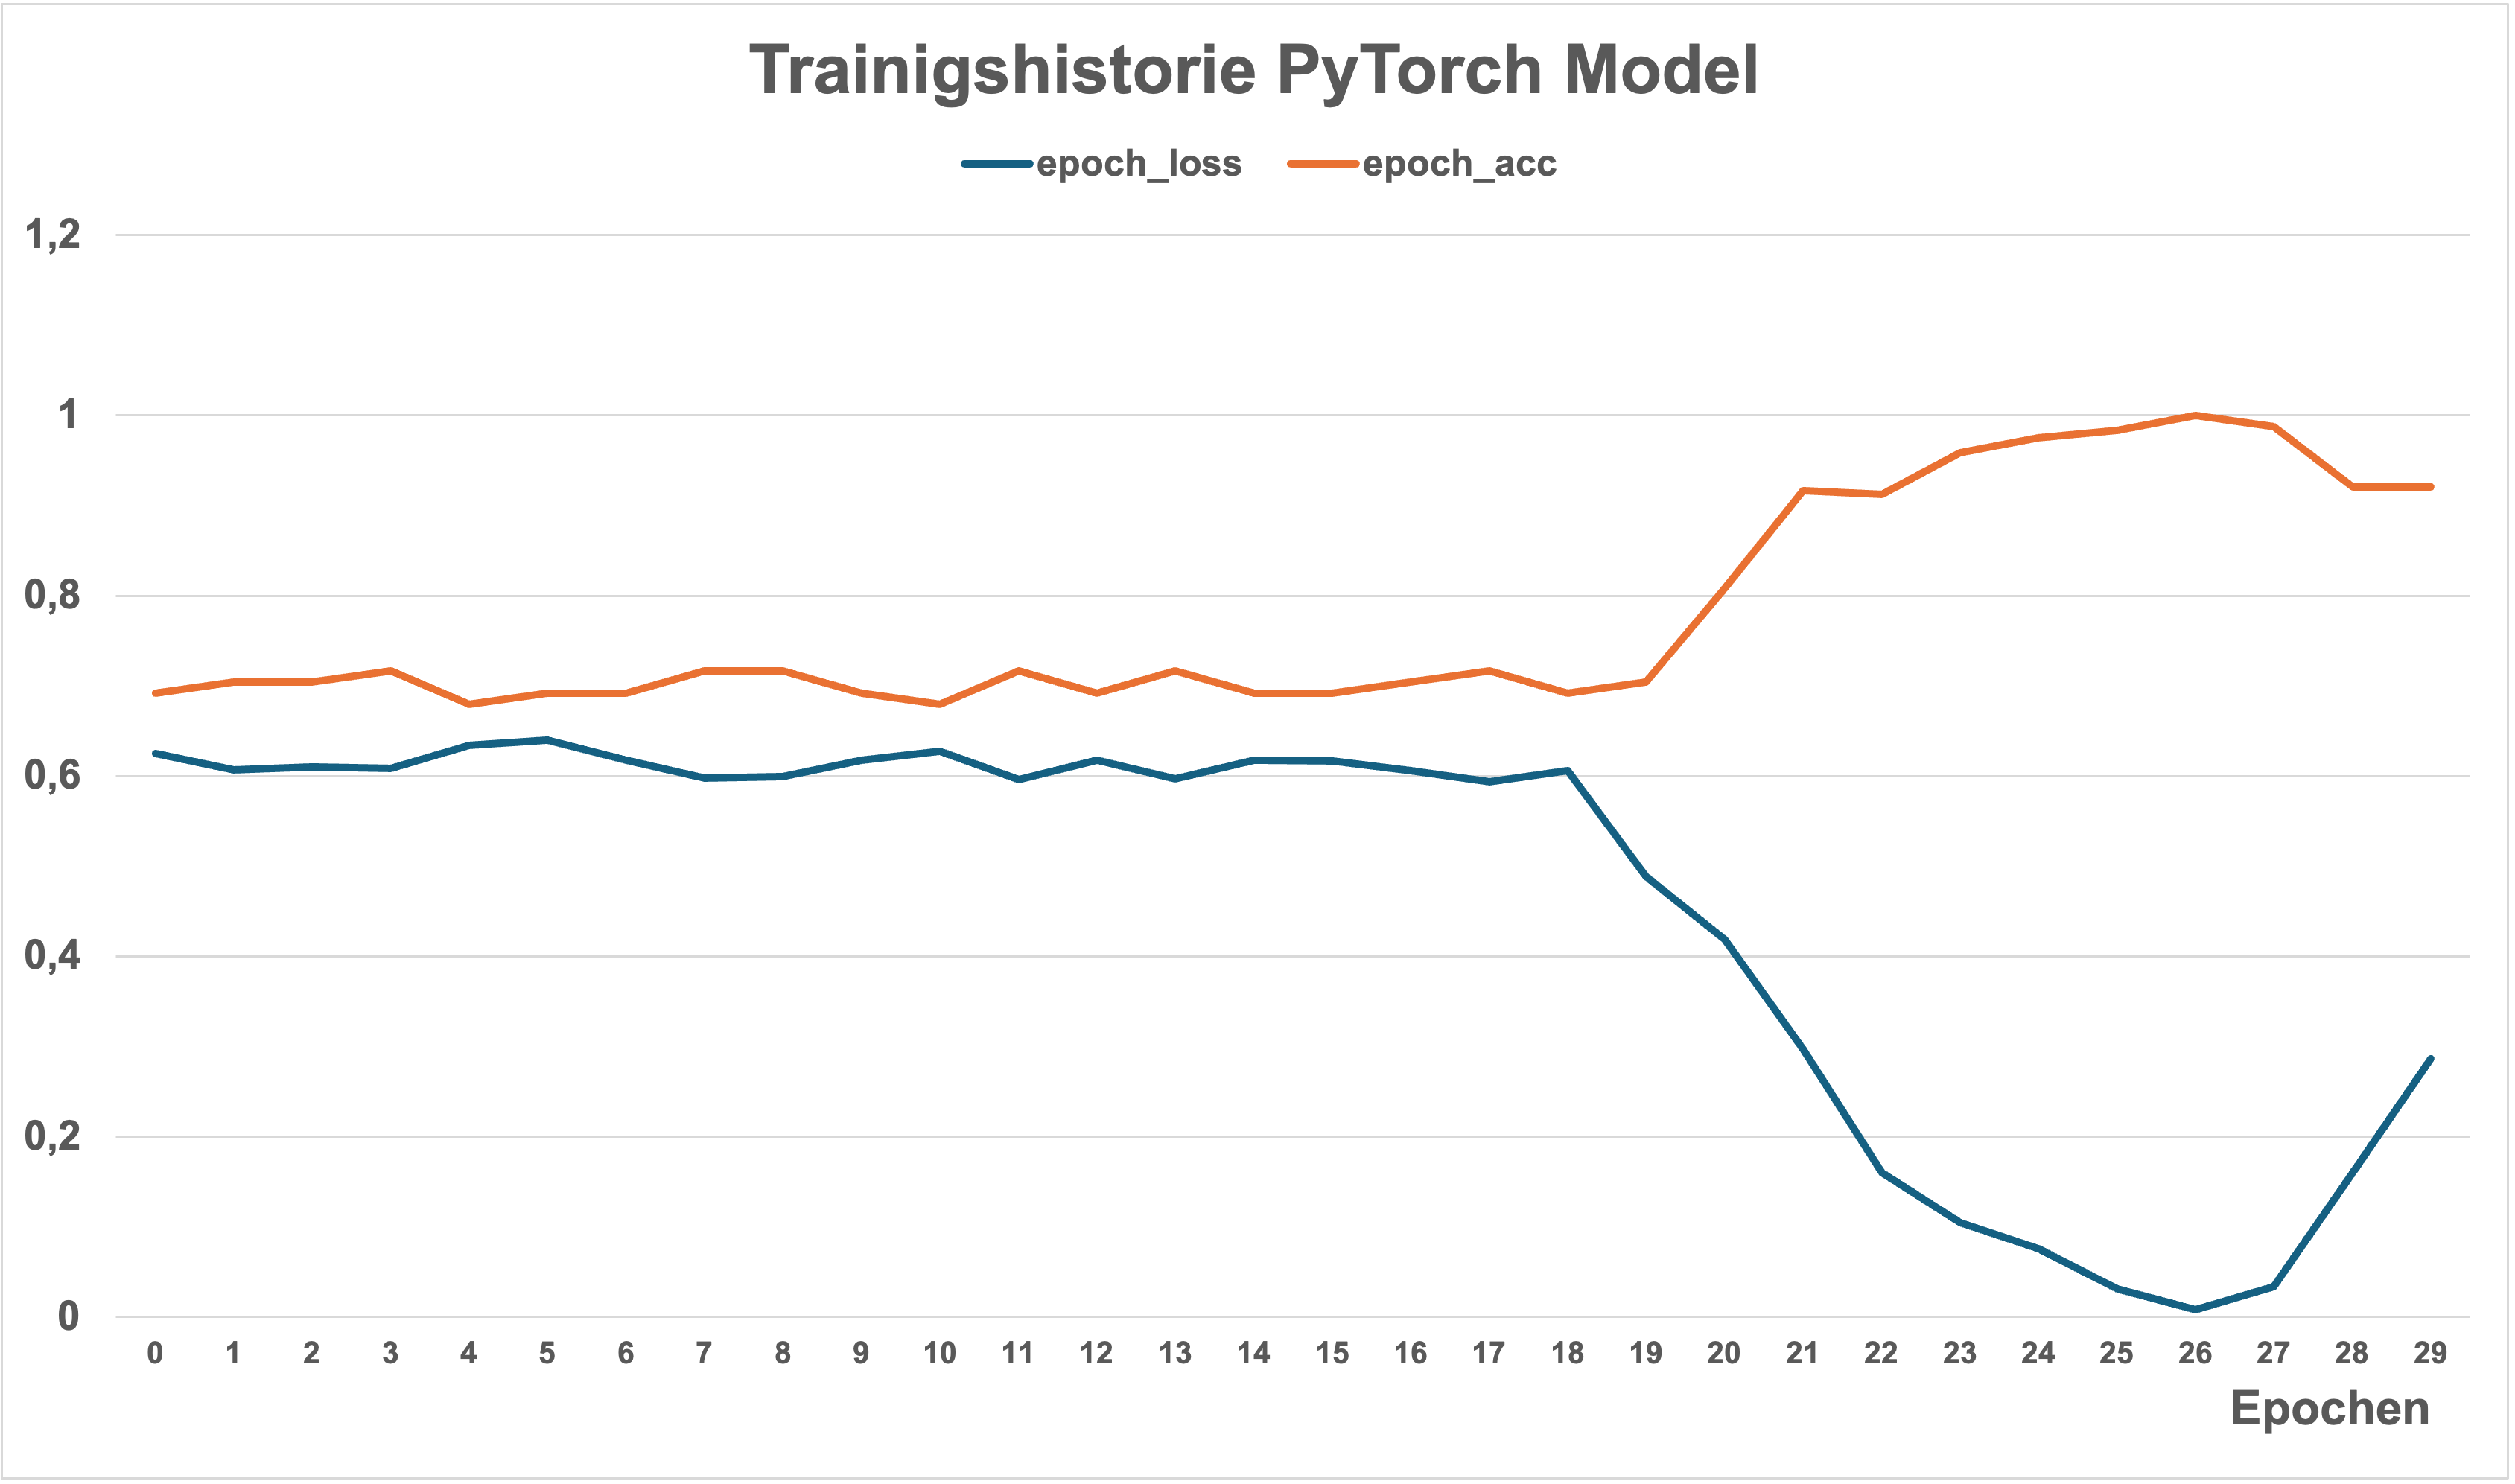
\includegraphics[width=1\textwidth]{Training_PyTorch.png}
    \caption{Schematischer Aufbau der API Kommunikation}
    \label{fig:Training_PyTorch}
\end{figure}

-Ergebnisse Vorstellen zwischen Selbstgeschriebenen Pytorch, Mobilenet und Mobilenet V3